\documentclass{beamer}

\usepackage{tikz}
\usepackage[labelfont=bf]{caption}
\usepackage{booktabs}
\usepackage{caption}
\usepackage{siunitx}
\usepackage{amsmath}
\usepackage{pgfplots}
\usepackage{pgfplotstable}

\title{Determining Acceleration due to Gravity through Sonic Time Measurements of Falling Masses}
\author{Henry Oehlrich\and Grace Jiang\and Ansh Agrawal}

\begin{document}
\maketitle

\begin{frame}
    \frametitle{Abstract}
    The objective of this experiment is to calculate the acceleration due to
    gravity. This was done using a sonic stopwatch to measure the time for
    varied masses to travel a vertical distance through a pulley. After
    multiple trials of different masses, acceleration due to gravity was
    calculated to be \qty{9.51}{\meter\per\second\squared}. 
\end{frame}

\begin{frame}
    \frametitle{Experiment Setup}
    \begin{minipage}{0.65\textwidth}
        \begin{figure}
            \centering
            \begin{tabular}{l|l|l}
                \toprule
                Symbol & Description &  Value \\
                \midrule
                $\Delta y$ & $m_2$ init height & \qty{1.70}{\meter} \\
                $m_1$ & constant mass & \qty{0.01}{\kilogram} \\
                $m_p$ & pulley mass & \\
                $r$ & pulley radius & \\
                $m_2$ & varied mass & varied \\
                $t$ & time & measured \\
            \end{tabular}
        \end{figure}
    \end{minipage}%
    \begin{minipage}{0.35\textwidth}
        \begin{figure}
            \centering
            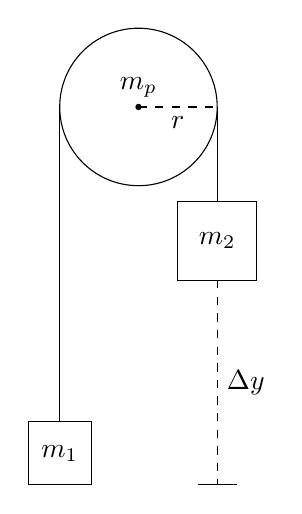
\begin{tikzpicture}
                \draw (0,5) node[above] {$m_p$} circle (1);
                \fill (0,5) circle (0.04);
                \draw[dashed] (0,5) -- (0.5, 5) node[below] {$r$} -- (1,5);
                \draw (1,5) -- (1,3.8);
                \draw (0.5,3.8) rectangle node {$m_2$} ++(1,-1);
                \draw (-1,5) -- (-1,1);
                \draw (-1.4,1) rectangle node {$m_1$} ++(0.8,-0.8);
                \draw[dashed] (1,2.8) -- (1,1.5) node[right] {$\Delta y$} -- (1,0.2);
                \draw (0.75,0.2) -- (1.25,0.2);
            \end{tikzpicture}
        \end{figure}
    \end{minipage}
\end{frame}

\begin{frame}
    \frametitle{Materials and Methods}
    The experiment setup consisted of two masses attached to dental floss
    strung over a ceiling mounted pulley. A hardcover book was used as a
    landing pad in order to dampen the collision and have consistent impact
    sounds. A \qty{0.01}{\kg} mass was hung at all times from one end of the
    dental floss. We conducted 7 trials for 5 larger masses hung from the other
    side of the dental floss. Time was measured using the Acoustic Stopwatch
    feature of phyphox. For each trial, the timer operator counted down and
    then snapped his fingers to activate the timer and alert the atwood
    operator to let go of the mass. The sound of the collision of the mass
    with the landing pad deactivated the timer.
\end{frame}

\begin{frame} 
    \frametitle{Results} 
    The data were arranged in a fashion which resulted in the calculated value
    of acceleration due to gravity to be the slope of the line of least
    squares. Through the regression, acceleration due to gravity was determined
    to be \qty{9.51}{\meter\per\second\squared}. The $R^2$ of
    \qty{99.2}{\percent} shows that only \qty{0.8}{\percent} of variance in net
    force is determined by the residuals; from this we can conclude that the
    timing method was negligibly inaccurate.
\end{frame}

\begin{frame}
    \frametitle{Linearized Graph}
    \centering
    \begin{tikzpicture}
        \begin{axis}[
                xlabel={$m_2 - m_1$ (\si{\kilogram})},
                ylabel={$F_s$ (\si{\newton})},
                xmin=0,xmax=0.1,
                ymin=0,ymax=1.1,
                tick label style={/pgf/number format/fixed},
                scaled ticks=false,
                width=0.8\textwidth
            ]
            \addplot +[only marks,mark size=1.5pt] table
            {xy.dat};
            \addplot table [
                y={create col/linear regression={y=force}},
                mark=none,
            ]
            {xy.dat};
            \addlegendentry{$F_s = a_s(m_2+m_1)$}
            \addlegendentry{$\hat{F_s} = \pgfmathprintnumber{\pgfplotstableregressiona}(m_2-m_1)$}
            \addlegendentry{$F_s = g(m_2-m_1)$}
        \end{axis}
    \end{tikzpicture}
\end{frame}

\begin{frame}
    \frametitle{Discussion}
    The value of acceleration due to gravity calculated in this experiment was
    \qty{9.51}{\meter\per\second\squared}. The accepted value of gravity is
    \qty{9.81}{\meter\per\second\squared}. The percent error of the measured
    value from the real value is \qty{3.1}{\percent}. The largest source of
    error was due to the internal friction of the plastic pulley provided. In
    the future, this error could be mitigated by using a more efficient pulley
    or by mathematically accounting for pulley friction. As explained in the
    Results section, there was negligible error in the measurement of time.
\end{frame}

\begin{frame}
    \frametitle{Acknowledgements}
    The authors would like to thank Mr. Grunden for introducing the acoustic
    stopwatch and for his invaluable guidance throughout the experiment.
\end{frame}

\end{document}
